\begin{flushleft}
    Die Wichtigste Anforderung an die Platform war, dass diese Modular aufgebaut werden kann. Denn dann ist es möglich, auch im Nachhinein
    neue Teile, Module oder komplett andere Sensoren einfach anzuschrauben, bzw. auch kaputte oder alte Teile problemlos zu erneuern.

    Da es sich beim Differentialantrieb nur um eine mechanische Anordnung der Motoren selbst handelt, musste noch ein
    geeignetes Bauteil als Motor selbst gefunden werden.
    Die Motoren müssen ein recht hohes Drehmoment, aber eine kleine Umdrehungszahl pro Minute aufweisen.
    Initial war es deshalb die Idee für normale 5V Motoren, wie sie auch in DVD Laufwerken verwendet werden, ein kleines
    Getriebe zu konzeptionieren und zu bauen, wie es in Abbildung \ref{fig:prototyp_transmission} zu sehen ist.

    \begin{figure}[h!]
        \centering
        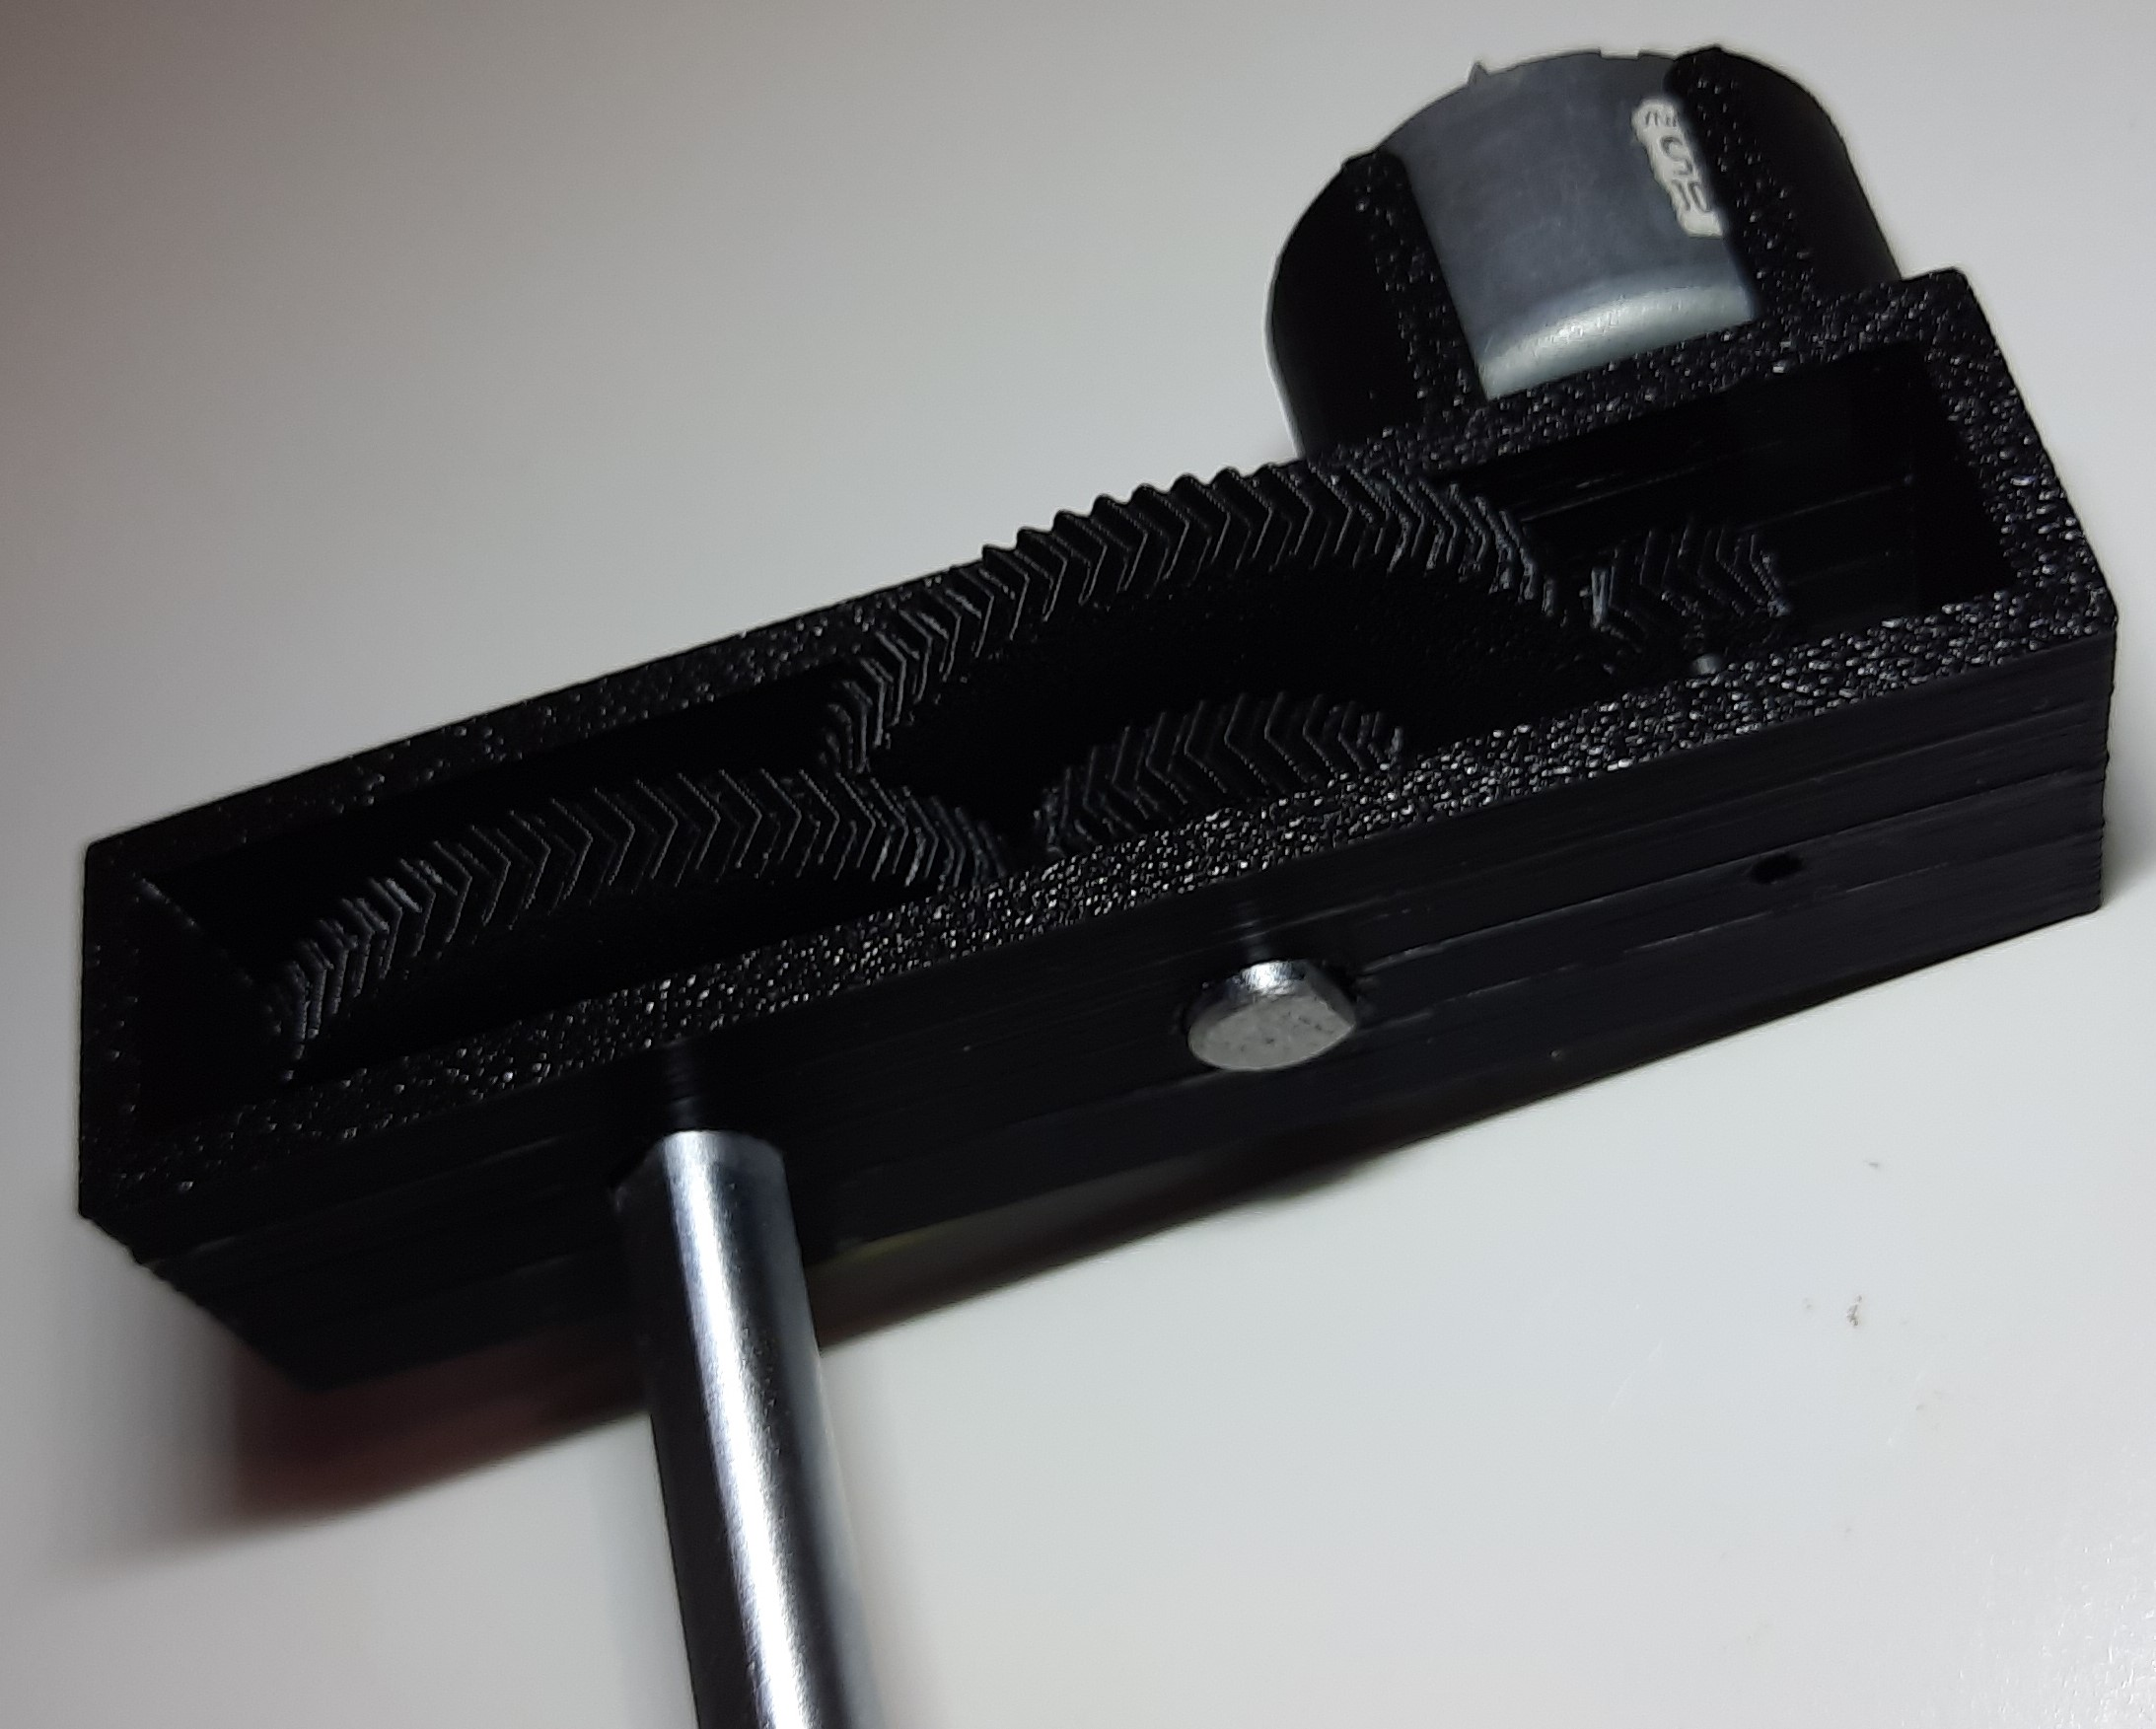
\includegraphics[width=0.3\textwidth]{imgs/Roboter/Real/Getriebe.jpg}
        \caption{Prototyp Eigenbau-Motorgetriebe}
        \label{fig:prototyp_transmission}%
    \end{figure}

    Die Idee bewies sich aber recht schnell als zu schwierig und wurde deshalb fallen gelassen.
    Als Ersatz für unseren misslungenen Versuch fiel die Entscheidung auf den Modellbau von Getriebemotoren (siehe Abbildung \ref{fig:robot_motor}).

    \begin{figure}[h!]
        \centering
        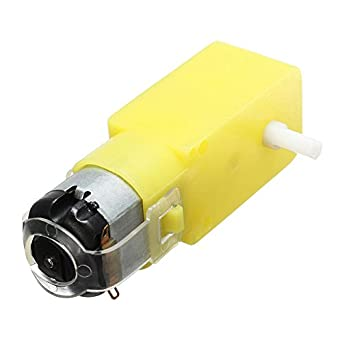
\includegraphics[width=0.3\textwidth]{imgs/Roboter/Real/41eJJZ8mOOL._SX342_.jpg}
        \caption{Modelbau Getriebemotor}
        \label{fig:robot_motor}%
    \end{figure}

    Ein Anforderung an unsere Demo Roboter Platform war die 3D-Druckbarkeit, sowie deren Modularer Aufbau.
    Das Fahrgestell unseres Roboters setzt sich aus insgesamt 3 Modulen zusammen.
    Die Motorenhalterung woran die Motoren selbst und auch die H-Brücke befestigt sind.
    Die Zentrale Platform für unseren Mikrocontroller.
    Und die beiden Freirollen an der Front des Roboters.

    Die gesamte Roboter Platform wurde mit Hilfe eines iterativen Design-Prozesses gestaltet. 
    Zu Begin wurde nur das Fahrgestell des Roboters designed und gedruckt (siehe Abbildung \ref{fig:cad_fahrgestell}).

    \begin{figure}[h!]
        \centering
        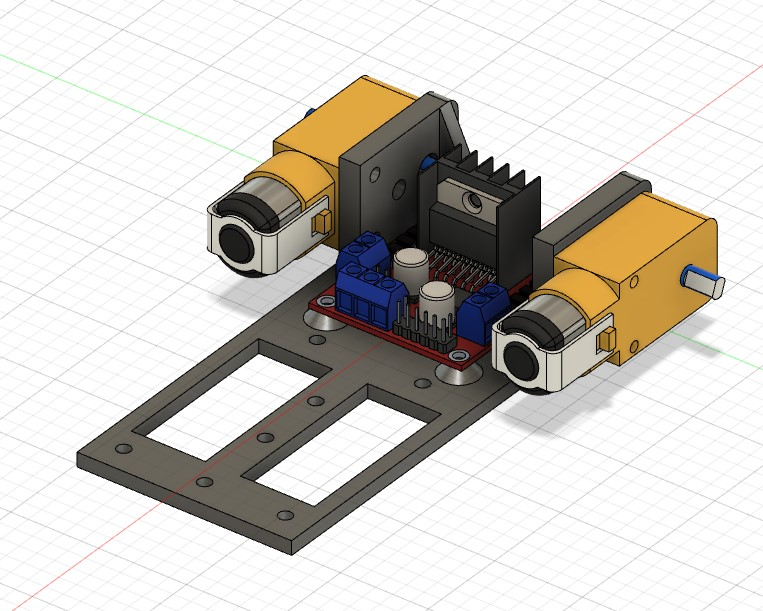
\includegraphics[width=0.3\textwidth]{imgs/Roboter/CAD/Fahrgestell.jpg}
        \caption{CAD Render vom finalen Fahrgestell}
        \label{fig:cad_fahrgestell}%
    \end{figure}

    Sobald das Ergebnis zufriedenstellend war wurde das nächste Modul designed und gedruckt.
    Dadurch erreichten wir eine Art Designkette und konnten sicherstellen das alle Teile bzw. Module zusammen passen
    und allen Anforderungen gerecht werden.
    Die letzten beiden Module für unseren Demo Roboter waren die Platform für die Elektronik (Abbildung \ref{fig:example} links) sowie die Freilaufrollen (Abbildung \ref{fig:example} rechts)
    an der Front des Roboters.

    \begin{figure}[h!]
        \centering
        \subfloat[\centering Elektronik Platform (finales Design)]{{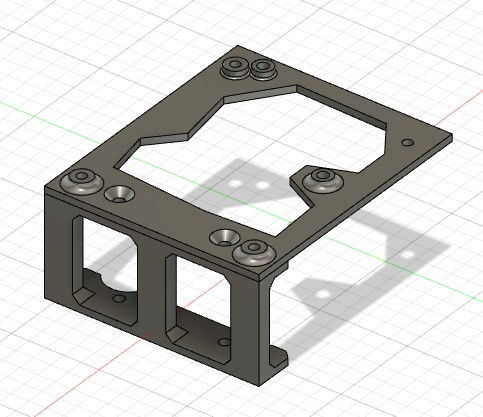
\includegraphics[width=0.3\textwidth]{imgs/Roboter/CAD/platform.jpg} }}%
        \qquad
        \subfloat[\centering Freilaufrollen (2. Version)]{{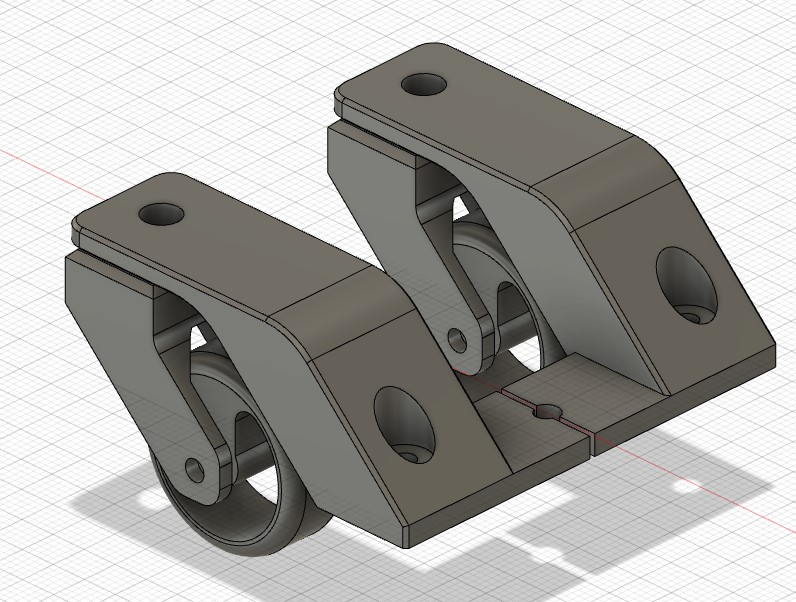
\includegraphics[width=0.3\textwidth]{imgs/Roboter/CAD/follower wheel.jpg} }}%
        \caption{CAD Render der Elektronik Platform und den Freilaufrollen}%
        \label{fig:example}%
    \end{figure}
\end{flushleft}